\newcommand{\scrartclScrreprt}{scrartcl}
%!TEX TS-program = pdflatex
\documentclass[numbers=noenddot,abstracton]{\scrartclScrreprt}

\usepackage[numbers]{natbib}
\usepackage[utf8x]{inputenc}
\usepackage[T1]{fontenc}
\usepackage{lmodern}
\usepackage{layout}
\setlength{\parindent}{0em}

\renewcommand{\baselinestretch}{1.2}
\renewcommand{\arraystretch}{1}

\let\oldmarginpar\marginpar
\renewcommand{\marginpar}[1]{\-\oldmarginpar[\raggedleft\scriptsize\hspace{0pt}#1]%
{\raggedright\footnotesize #1}}

%Damit \today ein Deutsch Formatiertes Datum zurueckgibt.  
\usepackage[ngerman, num, orig]{isodate}
\usepackage[ngerman]{babel}   

\monthyearsepgerman{\,}{\,} 

\usepackage{amssymb,amsmath,fancybox,graphicx,wrapfig,color,lastpage,fancyhdr,verbatim,epstopdf,a4wide}
\usepackage{paralist}	%aufzählungen in Tabelle machen

\usepackage{setspace}
\usepackage{epsfig}
\usepackage{supertabular}{\tiny }
\usepackage[font=small,labelfont=bf]{caption}
\usepackage{subcaption}
\usepackage{footnote}
\usepackage{float}
\usepackage{multirow}
\usepackage{etex}
\usepackage{pdfpages}
\usepackage{color} 
\usepackage{placeins} 
\usepackage{booktabs}


\usepackage[makeroom]{cancel}
\usepackage{array}
\usepackage{trfsigns}
\usepackage{textcomp}


% Kompaktes Itemize
\usepackage{enumitem}
\newlist{compactitemize}{itemize}{1}
\setlist[compactitemize]{label=\textbullet, nosep, leftmargin=10pt}


\usepackage{tikz}
\usetikzlibrary{shapes}
\usepackage{pgfplots}
\pgfplotsset{every axis plot/.style={line width=1pt}}
\pgfset{number format/1000 sep={}}
\pgfplotsset{tick label style={/pgf/number format/fixed}}
\pgfplotsset{scaled ticks=false}
\pgfplotsset{compat=newest}


\usepackage[hyphens]{url}	%URL handling und darstellung
\urlstyle{tt}

\usepackage[pdftitle={\titleinfo},
						pdfauthor={\authorinfo},
						pdfcreator={TeXStudio, LaTeX with hyperref},
						plainpages=false,
						pdfpagelabels,
						colorlinks,
						linkcolor=black,
						filecolor=black,
						citecolor=black,
						urlcolor=black]{hyperref}

\usepackage{tabularx}

\renewcommand{\captionfont}{\scriptsize\slshape}




\newcommand{\texttodo}[1]{\textcolor{red}{Todo: #1}}
\setlength{\unitlength}{1mm}

\setcounter{secnumdepth}{3}
\setcounter{tocdepth}{3}
	
%Abbildungsnumerierung anhand Kapitel
\renewcommand{\thefigure}{\arabic{section}.\arabic{figure}}
\makeatletter \@addtoreset{figure}{section} \makeatother

%%%%%%%%%%%%%%%%%%%%%%%%%%%%%%%%%%%%%%%%%%%%%%%%%%%%%%%%%%%%%%%%
% Begin define headings
%%%%%%%%%%%%%%%%%%%%%%%%%%%%%%%%%%%%%%%%%%%%%%%%%%%%%%%%%%%%%%%%
%\renewcommand{\headrulewidth}{0.4pt}
%\renewcommand{\footrulewidth}{0.4pt}

\lhead[\scriptsize\nouppercase{\leftmark}]{}%\textbf{\titleinfo}}
\chead[]{}
\rhead[]{\scriptsize\nouppercase{\leftmark}}%\textbf{\titleinfo}]{}

\lfoot[\scriptsize\thepage]{\scriptsize{}}
\cfoot[]{}
\rfoot[\scriptsize{}]{\scriptsize\thepage}

\AtBeginDocument{\numberwithin{equation}{section}} %Damit Gleichungen mit Section Nummer beginnen
\AtBeginDocument{\numberwithin{figure}{section}}
\AtBeginDocument{\numberwithin{table}{section}}



% Möglichst keine Ergänzungen hier, sondern in header.tex
\begin{document} 
 

% Römische Nummerierung für Sonderseiten, wie Verzeichnisse und Anhang
\pagenumbering{Roman}

% Titelblatt
\thispagestyle{empty}
\begin{center}
\begin{huge}
	\titleinfo
\end{huge}
\vfill
\begin{large}
\begin{tabular}{l p{0.5cm} l} 
  Fachgebiet & & \trfachgebiet \\ \vspace{0.2cm}
  Betreuung der Arbeit  & & \trprof \\   \vspace{0.2cm}
  Studiengang & & \trfakultaet \\ \vspace{0.2cm}
  Vorgelegt von & & \trauthorA $ $ und \trauthorB
\end{tabular}
\end{large}
\end{center}


\newpage
\renewcommand{\abstractname}{Abstract}
\begin{abstract}
Beispiel Text

\end{abstract}

\vspace{3cm}

% Inhaltsverzeichnis
\setcounter{tocdepth}{1}
\tableofcontents

% Nummerierung von roemisch auf arabisch umschalten und roemische
% zwischenspeichern
\newpage
\newcounter{roemisch}
\setcounter{roemisch}{\value{page}}
\pagenumbering{arabic}


\section{Aufgabenstellung}

\subsection{Aufgabe}
Das Licht nimmt immer den kürzesten Weg. Die Lichtgeschwindigkeit
h"angt von der optischen Dichte des Materials ab. Wie wird ein Lichtstrahl gekr"ummt, wenn die optische Dichte nicht konstant ist?

Die Natur regelt die Ausbreitung des Lichtes mit einem Minimumprinzip. Zeigen Sie, wie man aus diesem Minimumprinzip für die Ausbreitung von Lichtstrahlen zum Beispiel in einer Fata Morgana eine Differentialgleichung ableiten kann. Und auch das Brechungsgesetz von Snellius folgt aus diesem Optimumprinzip.

\section{Einleitung}
Wie in den vorangegangen Kapitel oft gesehen, stehen für Optimierungsprobleme verschiedene Programme wie z.B. der Symplex Algorithmus zur Verfügung. Dabei wird ein Maxima oder Minima gesucht. Bei der Variationsrechnung wird, wie in \chapref{chapter-variationsrechnung} beschrieben, eine Funktion gesucht welche, das Optimierungsproblem löst. Für die Variationsrechnung steht anstelle eines mathematischen Programms die Euler-Lagrange-Gleichung zur Verfügung. Wie nützlich und mächtig sie ist, soll anhand von Beispielen in folgenden Seiten etwas aufgezeigt werden.

\section{Einleitende Theorie, Fermatsches Prinzip}

Im Jahre 1660 fand Pierre de Fermat, ein Französischer Mathematiker, dass  nach ihm benannte, Fermatsche Prinzip heraus. 
Dieses lautet wie folgt \cite{DefinitionFermat}:

\begin{postulat}
	Der Weg, den das Licht nimmt, 
	um von einem Punkt zu einem anderen zu gelangen, 
	ist stets so, dass die benötigte Zeit minimal ist.
	\index{Fermatsches Prinzip 1}
\end{postulat}

Die \eqref{fermat} zeigt das Fermatsche Prinzip bei einem Brechungsindex $n$, 
der Lichtgeschwindigkeit $c$, dem Weg $s$ und dem Ort $r$ Die Zeit muss minimal sein.

\begin{align}
	t= \int\limits_{s_1}^{s_2} \frac{n(r)}{c} ds = \frac{1}{c} \int\limits_{s_1}^{s_2} n(r) ds
	\label{fermat}
\end{align}


Wenn die Zeit minimal ist, wird bei kleinen Abweichungen vom Weg die Zeit nicht viel grösser. 
Deshalb kann die oben stehende Definition auch wie folgt geschrieben werden\cite{Definition}.

\begin{postulat}
Der Weg, den das Licht nimmt,  um von einem Punkt zu einem anderen zu gelangen, 
ist stets so, dass die Zeit, die das Licht benötigt, invariant gegen kleine Änderungen des Weges ist.
\index{Fermatsches Prinzip 2}
\end{postulat}

\subsection{Formulierung mit dem optischen Weg}
Der optische Weg $L$  eines Pfades $s$ kann in einem homogenen Material 
mit dem Brechungsindex $n$ als Produkt von $n$ und $s$ berechnet werden.
Bei einem inhomogenen Material ergibt sich für den optischen Pfad die allgemeine \eqref{optischweg}.
\begin{align}
	L(s) = \int\limits_{s_1}^{s_2} n(r) \,\mathrm d\vec s 
	\label{optischweg}
\end{align}

Da der zurückgelegte Weg des Lichtstrahles direkt proportional zur Zeit ist, $s = c \cdot t$,
und das Licht sich in optisch dichteren Materialien langsamer bewegt,
kann das Fermatsche Gesetz umformuliert werden\cite{Definition}. 


\begin{postulat}
Der Weg, den das Licht nimmt, um von einem Punkt zu einem anderen zu gelangen, ist stets so, dass der optische Weg minimal ist.
\index{Fermatsches Prinzip 2}
\end{postulat}

\subsection{Erklärung}
Viele Leute haben ein Problem mit dem Fermatschen Prinzip. 
Der Grund ist ganz einfach. 
Bei der ``klassischen'' Strahlenoptik geht das Licht einen bestimmten Weg, 
sieht einen Spiegel oder eine Oberfläche, bricht sich dort nach einem 
physikalischen Gesetz und geht dann weiter.
Der philosophische Ansatz vom Fermatschen Prinzip ist anders. 
Es wird davon ausgegangen, dass das Licht, bevor es einen Weg einschlägt, 
weiss wohin es muss. Es weiss, wo ein Spiegel oder eine Oberfläche kommt und 
nimmt dem entsprechend von Anfang an den Weg mit der kürzesten Zeit.
Aber woher weiss das Licht, dass sein eingeschlagener Weg der korrekte ist?
Kann man davon ausgehen, dass es die nähere Umgebung anschaut und diese Vergleicht?
Ja, genau davon kann man ausgehen. Eine mögliche Erklärung mit Hilfe von Elektromagnetischen Wellen ist,
dass sich das Licht in alle Richtungen ausbreitet. 
Jedoch interferieren die meisten dieser Wellen destruktiv, 
ausser die Welle, welche den Weg mit der kürzester Zeit genommen hat, wird nicht ausgelöscht.

\section{Rechnung an einem Konkreten Beispiels}

\subsection{Brechungsgesetz von Snellius \label{brechungsgesetz}}
\cite{Wikipedia} Aus dem Fermatschen Prinzip lässt sich das Brechungsgesetz von Snellius herleiten.
Das Licht legt den Weg vom Startpunkt $P_0$ über den Brechungspunkt $P_1$ 
nach dem Endpunkt $P_2$ zurück, siehe \figref{Ab:brechung}.
\begin{figure}[H]
	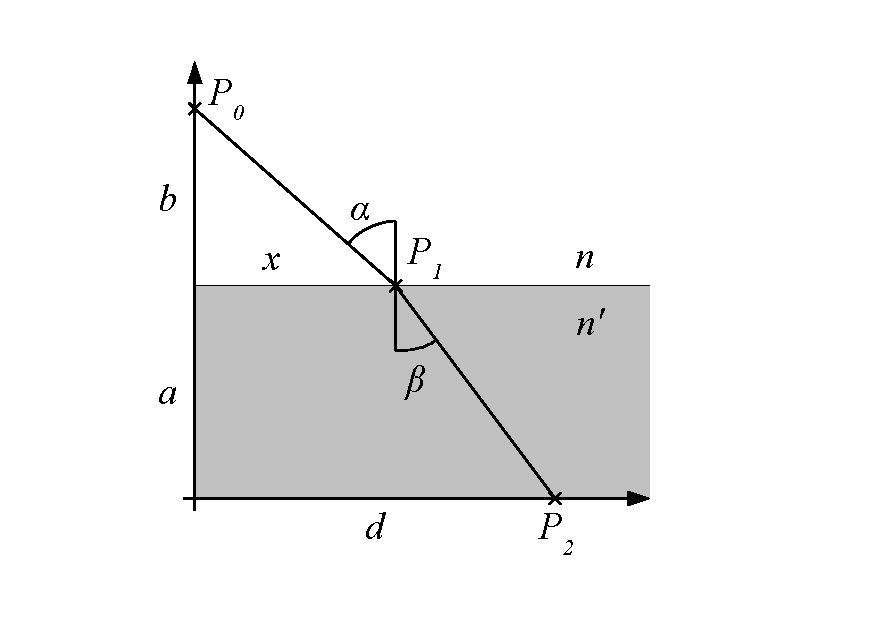
\includegraphics[width=0.8\textwidth]{./picture/Brechung.pdf}
	\caption{Skizze des Brechungsgesetzes von Snellius}
	\label{Ab:brechung}
\end{figure}

Dadurch kann die zurückgelegte Zeit berechnet werden (\eqref{snelliusT}).
\begin{align}
t(x) = t_1 + t_2 = \frac{s_1}{c_1} + \frac{s_2}{c_2} = \frac{|P_1 - P_0|}{c_1} + \frac{|P_2 - P_1|}{c_2} \notag \\
= \frac{\sqrt{a^2 + x^2}}{c_1} + \frac{\sqrt{(d-x)^2 + b^2}}{c_2} \label{snelliusT}
\end{align}

Wird diese Funktion nach $dx$ abgeleitet und gleich Null gesetzt wird die Extremastelle von $t$ gefunden (\eqref{snelliusDx}).
\begin{equation}
	\frac{dt}{dx} = \frac{2 \cdot x}{2 \cdot c_1 \cdot \sqrt{a^2 + x^2}} + \frac{-2 \cdot (d-x)}{2 \cdot c_2 \cdot \sqrt{(d-x)^2 + b^2}} =
	\frac{x}{c_1 \cdot \sqrt{a^2 + x^2}} - \frac{(d-x)}{c_2 \cdot \sqrt{(d-x)^2 + b^2}} = 0 \label{snelliusDx}\\
\end{equation}

Eine weitere Ableitung und einsetzen von $x_0$ welches beim berechnen von (\eqref{snelliusDx}) gefunden wird zeigt ob ein lokales Maxima oder Minima vorliegt.
\begin{align}
\text{mit} c_2=2 \cdot c_1 \qquad a=1 \qquad b=2a \qquad d=1 \textbf{ist} x_0 = 0.190898 \notag \\
\frac{dt}{d^2x}=\frac{1}{c2 \sqrt{b^2 + (d - x)^2}} - \frac{(d - x)^2 }{c2 (b^2 + (d - x)^2)^(3/2)} \notag \\
- \frac{x^2}{c1 (a^2 + x^2)^(3/2)} + \frac{1}{c1 \sqrt{1^2 + x^2}} = y  \notag \\
y =\frac{1.14688}{c1} > 0
\end{align}
$x_0$ ist lokales Minima, da es auch der einzige Kandidat für eine Extremastelle ist, ist es auch ein globales Minimum.



Aus \figref{Ab:brechung} ist gut ersichtlich das die Substitutionen \ref{substitution1} und \ref{substitution2} durchgeführt werden können,

\begin{align}
	\sin(\alpha) = \frac{x}{\cdot \sqrt{a^2 + x^2}}  \label{substitution1}\\
	\sin(\beta) = \frac{d-x}{\sqrt{(d -x)^2 + b^2}} \label{substitution2}
\end{align}

Nach etwas umformen ergibt sich, das Verhältnis der Winkel $\alpha \ \text{und} \ \beta$ gemäss (\eqref{snellius}).

\begin{equation}
	0 = \frac{\sin(\alpha)}{c_1} - \frac{\sin(\beta)}{c_2} \Leftrightarrow\frac{c_2}{c_1} = \frac{\sin(\beta)}{\sin(\alpha)}
	\label{snellius}
\end{equation}


\subsection{Reflexionsgesetz}
\cite{Wikipedia} Auf gleiche weise wie das das Brechungsesetz aus dem Fermatschen Prinzip hergeleitet wird, 
lässt sich daraus auch das Reflexionsgesetz ableiten.
Das Licht legt den Weg vom Startpunkt $P_0$ über den Spiegelpunkt $P_1$ 
nach dem Endpunkt $P_2$ zurück. Dadurch kann die zurückgelegte Zeit berechnet werden (\eqref{reflexion}).


\begin{align}
t(x) = t_1 + t_2 = \frac{s_1 + s_2}{c} = \frac{|P_1 - P_0| + |P_2 - P_1|}{c} \notag \\
= \frac{\sqrt{a^2 + x^2} + \sqrt{(d-x)^2 + b^2}}{c} \label{reflexion}
\end{align}

Wenn $t(x)$ nach $dx$ abgeleitet und gleich 0 gesetzt wird ergibt sich die Extremastelle  von $t$ (\eqref{reflexionDx}). Auf den Beweis das es ebenfalls ein Minimum ist wie bei der Reflexion wird hier verzichtet.

\begin{align}
\frac{dt}{dx} = \frac{1}{c} \cdot \frac{2 \cdot x}{2 \cdot \sqrt{a^2 + x^2}} + \frac{-2 \cdot (d-x)}{2 \cdot \sqrt{(d-x)^2 + b^2}} \notag \\
= \frac{x}{ \sqrt{a^2 + x^2}} - \frac{(d-x)}{ \sqrt{(d-x)^2 + b^2}} = 0 \label{reflexionDx}
\end{align}

\begin{figure}[H]
	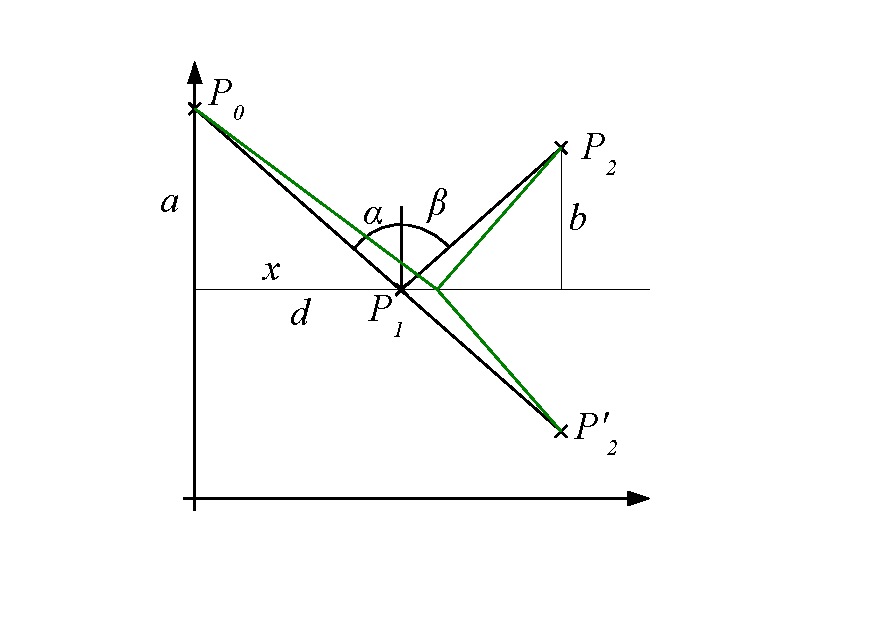
\includegraphics[width=0.8\textwidth]{./picture/Spiegelung.pdf}
	\caption{Skizze des Reflexionsgesetzes}
	\label{Ab:spiegelung}
\end{figure}

In \figref{Ab:spiegelung} ist ersichtlich, dass die Substitutionen \ref{substitution1} und \ref{substitution2} von \secref{brechungsgesetz} auch hier nützlich sind.
Nach etwas umformen ergibt sich, dass Eintritts- und Austrittswinkel gleich sind (\eqref{brechung}).


\begin{equation}
0 = \sin(\alpha) - \sin(\beta) \Leftrightarrow \sin(\beta) = \sin(\alpha) \Leftrightarrow\beta = \alpha
\label{brechung}
\end{equation}

In \figref{Ab:spiegelung} ist ersichtlich, dass die Linie des Startpunktes bis zum 
gespiegelten Endpunkt eine Gerade ist, welche der Funktion des kürzesten Weges entspricht.



\end{document}


